\section{Существующие решения}
Задача профилирования не нова.
Профилировщики разного уровня сложности существовали с самой зари программирования.
Рассмотрим некоторые важные для постановки задачи существующие решения, проанализируем их подходы, преимущества и недостатки.

\subsection{Метрики}
При оптимизации программ крайне важно сформулировать метрику, которую планируется улучшить.
Для разных видов метрик существуют различные решения для профилирования.
Можно выделить несколько наиболее востребованных метрик.

\subsubsection{Реальное время}
Программа, использующая меньше реального времени (wall time, <<время по настенным часам>>),
быстрее генерирует результат и быстрее отвечает пользователю.
Для оптимизации реального времени, например, убирают лишние взаимодействия с дисковой или сетевой подсистемами,
делают их асинхронными, избавляются от тяжелых взаимных блокировок потоков,
повышают утилизацию вычислительных мощностей, разбивают однопоточные вычисления на несколько потоков.

\subsubsection{Процессорное время}
Оптимизация CPU time в общем случае отличается от оптимизации Wall time.
Часто повышение пропускной способности системы понижает ее отзывчивость, и наоборот.
В то же время, некоторые оптимизации позволяют сэкономить и CPU time, и Wall time, например, использование более эффективных однопоточных алгоритмов.
Система, потребляющая меньше количество CPU time, более экономна и позволяет обработать больше запросов за единицу времени.
В рамках данной работы рассматривается в первую очередь оптимизация процессорного времени.

\subsubsection{Анонимная память}
Анализ использования оперативной памяти программой зачастую не менее важен, чем анализ использования CPU.
К сожалению, в отличие от CPU time и Wall time, использование анонимной оперативной памяти
отлаживать достаточно сложно. Современные программы используют нетривиальные аллокаторы
в качестве прослойки между пользовательским кодом и операционной системой, скрывающие большое
количество нюансов при работе с памятью и эффективно переиспользующих регионы памяти.

Существует ряд удобных инструментов для анализа использования памяти \cite{valgrind, gperftools, tcmalloc:hp}, однако
применяемые там техники достаточно специальны и мало применимы в нашем случае.

\subsubsection{Низкоуровневые события}
Широко распространенные архитектуры процессоров (x86-64, ARM, IBM POWER9, RISC-V и другие)
поддерживают механизмы эффективного получения различных счетчиков производительности
напрямую с процессора при помощи особого набора инструкций.
Устройство, отвечающее за отслеживание и обработку событий, известно как Performance Monitoring Unit (PMU).

В качестве счетчиков могут выступать произвольные события, интересные инженерам.
Например, количество тактов процессора, количество промахов кеша второго уровня или количество
инструкций ветвления, предугаданных механизмом предсказания ветвлений.
Кроме того, зачастую поддерживается механизм семплирования \cite{linux:pmi}, при котором процессор генерирует
особое прерывание при переполнении счетчика. Ядро операционной системы обрабатывает
данное прерывание и анализирует состояние системы на момент прерывания.

Данный механизм позволяет получать статистическое приближение реального распределения использования тех или иных ресурсов.

\subsection{Раскрутка стека}
Подавляющее большинство профилировщиков при анализе собирают информацию о стеке вызовов функций программы.
Это позволяет изучать не только функции-листья, в которых не происходит вызовов других функций, но и тяжелые промежуточные функции,
что значительно повышает применимость и удобство использования профилировщика.
Например, само по себе появление функции \verb!memcpy! в профиле значит мало: важен контекст ее вызова.
Рассмотрим различные варианты получения стеков потоков.

\subsubsection{Frame pointers}
Наиболее примитивной методикой получения стека является раскрутка с использованием frame pointers.
На x86-64 в этом режиме пролог и эпилог каждый функции выглядит стандартным образом:
\begin{verbatim}
foo:
    push %rbp
    mov %rsp, %rbp
    ...
    mov %rbp, %rsp
    pop %rbp
    ret
\end{verbatim}
При этом \verb!rbp! --- регистр стекового кадра, изменение \verb!rbp! внутри тела функции запрещено.
Важно, что \verb!rbp! callee-saved регистр, то есть, дочерние функции обязаны сохранить значение регистра после возврата.

Если все функции в программе скомпилированы с данным прологом и эпилогом,
то, зная текущее значение регистра \verb!rbp!, легко восстановить весь стек вызовов: все сохраненные на стек в прологе функций
значения \verb!rbp! образуют связный список; значения адресов возврата тривиально вычисляются на основе значения регистра стекового кадра.

\begin{figure}[H]
    \centering
    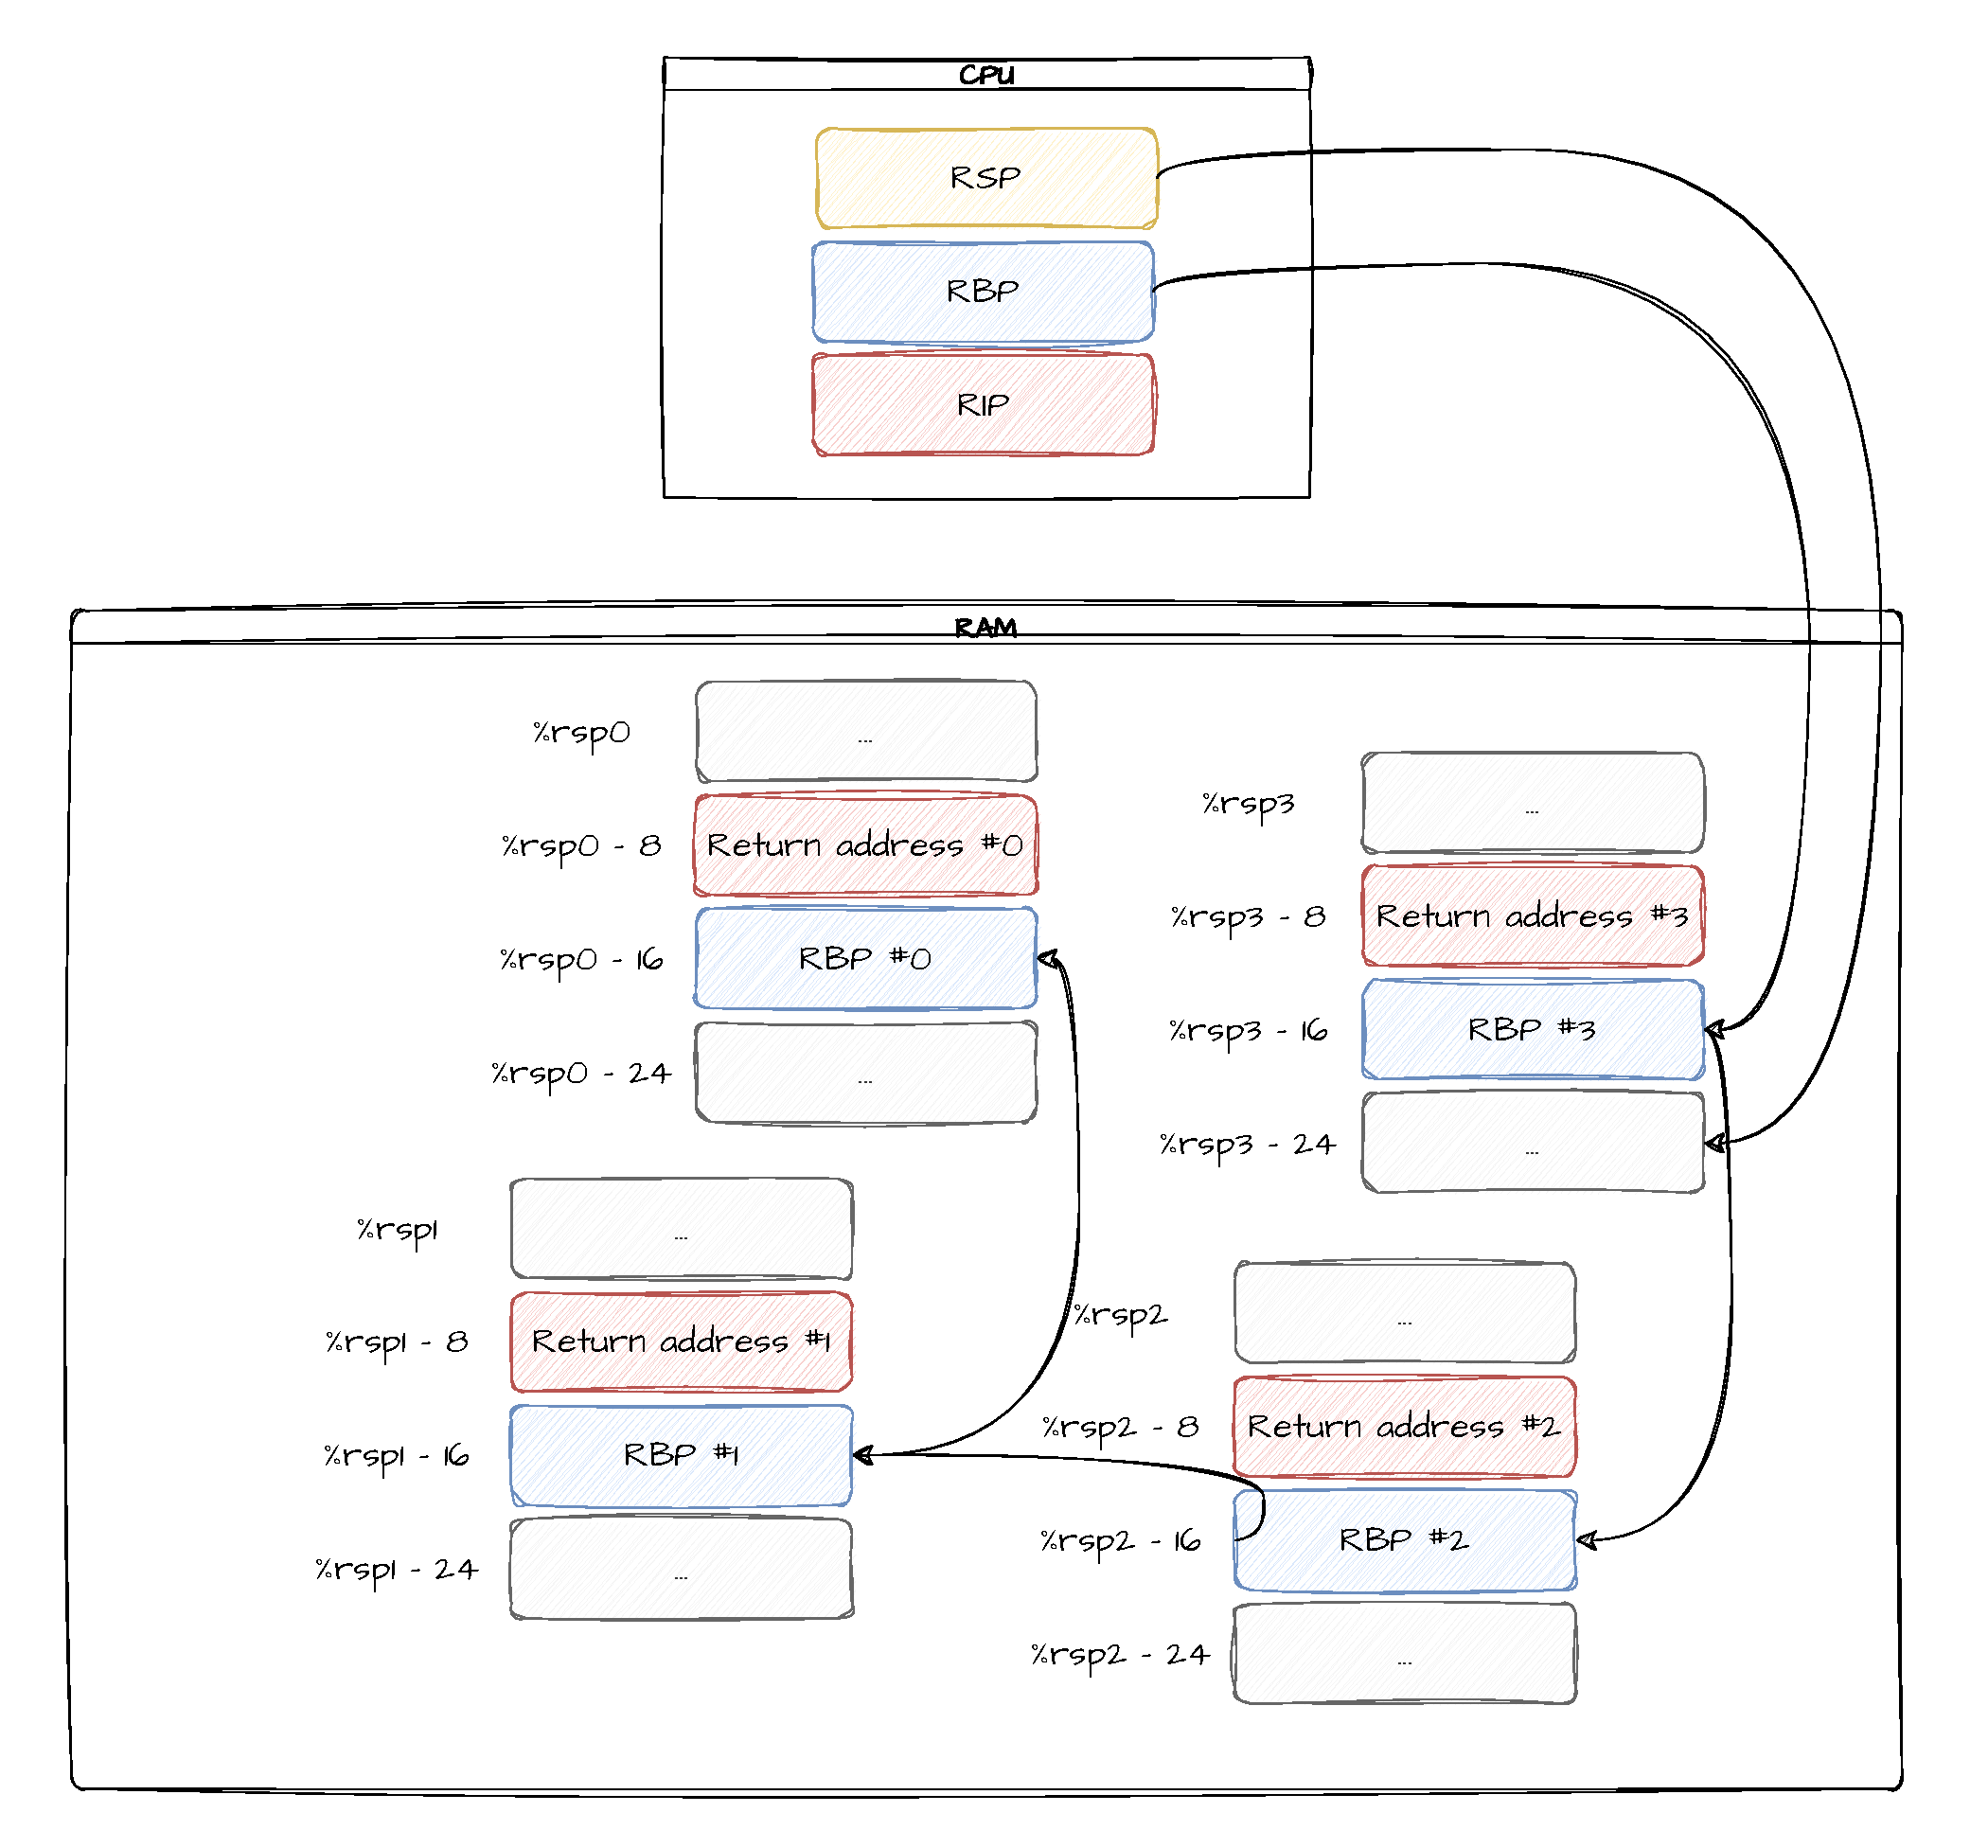
\includegraphics[width=\textwidth]{frame-pointers.pdf}
    \caption{Пример состояния регистров и стека процесса}
    \label{fig:fp}
\end{figure}

К сожалению, в настоящее время данный режим используется достаточно редко.
Современные оптимизирующие компиляторы по умолчанию не генерируют пролог и эпилог функций,
что позволяет сэкономить на использовании регистра \verb!rbp! исключительно для целей организации стековых кадров.
Эффект от наличия дополнительного регистра сложно оценить.
На практике при включении опции компилятора, требующей генерировать стандартный пролог и эпилог для всех функций
(\verb!-fno-omit-frame-pointer!), производительность различных программ уменьшается на 2-10\%.
Масштабное обсуждение данной проблемы приведено в \cite{fp:fedora}.

\subsubsection{LBR}
Компания Intel предоставляет в своих процессорах возможность запоминать адреса нескольких последних инструкций ветвления:
механизм LBR (last branch record). LBR записывается в набор MSR (model specific register).
Для каждой записи в журнале выделено три MSR: адрес исходной инструкции, адрес инструкции назначения и регистр с метаинформацией.
В метаинформации, например, отражен результат предсказания процессором поведения данной инструкции ветвления.
Для активации LBR достаточно установить особый бит в управляющем MSR.
Для уменьшения влияния LBR на производительность процессора механизм LBR сохраняет не все инструкции ветвления, а некоторое подмножество,
выбираемое через равные промежутки циклов процессора.

Кроме того, механизм LBR позволяет настроить запись не просто произвольных инструкций ветвления, но исключительно инструкций
вызова подпрограммы и выхода из нее (\verb!call! и \verb!ret!).
В данном режиме \verb!ret! удалят последнюю запись в журнале, что позволяет получать примерное представление о стеке вызовов.

Современные процессоры (Intel Skylake и новее) поддерживают до 32 записей в журнале LBR;
более ранние поколения микроархитектуры поддерживают 4, 8 или 16 (Nehalem – Haswell) записей \cite{lbr:lwn}.
Такое количество записей уже достаточно нетривиально в реализации на кристалле процессора,
так как на каждую запись в журнале LBR необходимо выделить три регистра (24 байт).
Однако, для задачи раскрутки стека в профилировщике даже 32 записей недостаточно: реальные стеки программ зачастую в разы глубже.

\subsubsection{DWARF}
На самом деле, задача точной раскрутки стека давно решена.
Через данный механизм работают отладчики и, например, известные реализации рантайма языка C++,
раскручивающие стек вызовов функции при выбросе исключения (Itanium C++ ABI \cite{itanium:eh}).

Раскрутка стека в обоих случаях происходит при использовании одной из двух специальных секций в исполняемом файле ---
в полной \verb!.debug_frame! и урезанной \verb!.eh_frame!.
Обе секции хранятся в крайне сложном формате отладочной информации DWARF CFI \cite{dwarf}.

В описываемых секциях хранятся сильно сжатые структуры данных, позволяющие из любой точки программы вычислить
состояние родительского стекового кадра. Основное отличие \verb!.debug_frame! и \verb!.eh_frame! --- объем восстанавливаемой информации.
Первая позволяет вычислить состояние всех регистров на момент вызова дочерней функции, вторая --- только базового набора регистров,
необходимых для раскрутки стека.
Кроме того, зачастую секцию \verb!.debug_frame! удаляют из релизных версий исполняемых файлов для уменьшения их размера
(например, при помощи инструмента \verb!strip!), в то время как от наличия секции \verb!.eh_frame!
зависит корректность исполняемого кода. Без данной секции невозможен процесс выброса исключений.
Более того, секция \verb!.eh_frame! по умолчанию генерируется даже для бинарных файлов, не использующих исключения;
отключить ее создание можно при помощи флага \verb!-fno-asynchronous-unwind-tables! в GCC или Clang, однако на практике
данный режим используется достаточно редко.
Таким образом, при разработке профилировщика мы можем предполагать, что с большой вероятностью отлаживаемый бинарный файл содержит
секцию \verb!.eh_frame!.

Одним из существенных недостатков подхода с раскруткой через \verb!.eh_frame! является отсутствие информации для раскрутки стека
при написании кода на языке ассемблера вручную. В качестве решения современные ассемблеры поддерживают набор директив CFI, позволяющих
вручную размечать свой код для целей раскрутки \cite{cfi:directives}.

Важно, что помимо данных секций, в формате DWARF хранится большое количество дополнительной отладочной информации;
например, отображение из адреса инструкции в имя функции, содержащей данную инструкцию.

Рассмотрим подробнее процесс раскрутки стека с использованием секции \verb!.eh_frame!.
Секция состоит из набора структур Common Information Entry (CIE) и Frame Description Entry (FDE).
Первая структура описывает несколько служебных полей; почти вся информация, необходимая для раскрутки стека, находится в FDE.
Каждой функции соответствует ровно одна из записей FDE.
Каждая FDE содержит список строк, где каждая сильно сжата (хранятся только изменения относительно предыдущей, сами изменения кодируются
стандартным для DWARF механиками с использованием виртуальный машины DWARF).
Каждой строке соответствует несколько подряд идущих инструкций в машинном коде программы. Строка описывает, как для любой из инструкций,
принадлежащих строке, восстановить адрес стекового кадра функции (CFA, Canonical Frame Address),
найти адрес возврата из текущей функции и восстановить несколько важных для раскрутки регистров.

Например, для фрагмента кода
\begin{verbatim}
0000000000041370 foo:
 * 41370:	push   %rbp
 * 41371:	push   %rbx
 * 41372:	mov    %rdi,%rbx
   41375:	sub    $0x18,%rsp
 * 41379:	mov    %fs:0x28,%rax
   41382:	mov    %rax,0x8(%rsp)
   41387:	lea    0x15082(%rip),%rax
    ...
   413d2:	jne    4143e
   413d4:	add    $0x18,%rsp
 * 413d8:	pop    %rbx
 * 413d9:	pop    %rbp
 * 413da:	ret
\end{verbatim}

Возможна генерация следующей таблицы FDE:
\begin{table}[H]
\begin{center}
\begin{tabular}{ |c||c|c|c|c| } 
 \hline
Instruction address   & CFA    & rbx    & rbp    & Return address \\
 \hline
0x41370 & rsp+8  & undef  & undef  & CFA-8 \\
0x41371 & rsp+16 & undef  & CFA-16 & CFA-8 \\
0x41372 & rsp+24 & CFA-24 & CFA-16 & CFA-8 \\
0x41379 & rsp+48 & CFA-24 & CFA-16 & CFA-8 \\
0x413d8 & rsp+24 & CFA-24 & CFA-16 & CFA-8 \\
0x413d9 & rsp+16 & CFA-24 & CFA-16 & CFA-8 \\
0x413da & rsp+8  & CFA-24 & CFA-16 & CFA-8 \\
 \hline
\end{tabular}
\end{center}
\caption{Пример FDE}
\end{table}

Астерисками в исходном коде помечены те инструкции, которые генерируют новые строки в FDE.

Теперь, зная структуру FDE, восстановление предыдущего стекового кадра достаточно тривиально:
необходимо вычислить значение CFA из второй колонки FDE, после чего на основе CFA пересчитать значения rbx и rbp.

К сожалению, потенциальная структура FDE заметно сложнее приведенной:
DWARF позволяет использовать Тьюринг-полные выражения для вычисления состояния регистров \cite{dwarf:turingcomplete}.
Рассмотрение стековой виртуальной машины DWARF выходит за рамки данной работы,
однако приведем пример некоторых реально используемых сложных выражений для раскрутки стека:
\begin{verbatim}
DW_OP_breg7 RSP+8
DW_OP_breg16 RIP+0
DW_OP_lit15
DW_OP_and
DW_OP_lit10
DW_OP_ge
DW_OP_lit3
DW_OP_shl
DW_OP_plus
\end{verbatim}
Что на псевдокоде выглядит как \verb!rsp + 8 + (((rip & 0xf) >= 0xb) << 3)!.
Данное правило вычисления CFA используется в \verb!.plt! секциях, используемых при динамическом связывании.

\subsubsection{SFrame}
В настоящее время Indu Bhagat из Oracle разрабатывает альтернативу раскрутке стека
через DWARF CFI: SFrame \cite{sframe:phoronix, sframe:lwn}.
Это компактный формат, основанный на более раннем формате ORC (был разработан специально для нужд ядра Linux \cite{orc}),
приспособленный исключительно для раскрутки стека профилировщиками и отладчиками.
SFrame хранится в отдельной загружаемой секции бинарных файлов ELF.
SFrame с недавнего времени поддержан в GNU Binutils \cite{sframe:commits}.

В мае 2023 года Indu предложил патч в ядро Linux, поддерживающий новый формат раскрутки в подсистеме perf, на которой
основаны современные профилировщики под Linux (подробнее о perf в \ref{sec:perf}).
К сожалению, патч достаточно нетривиальный, и изменение, хоть и было воспринято позитивно, вряд ли быстро окажется доступным пользователям.
Основная проблема – необходимость обрабатывать и анализировать секцию \lstinline!.sframe! без замедления
старта всех процессов в системе \cite{sframe:ml}. Предлагаемое ленивое решение не подходит для общего случая, так как при первом доступе в
структуру \lstinline!.sframe! системе придется вычитать секцию с диска, что неприемлемо в условиях работы профилировщика (при прерывании).

Секции с SFrame вряд ли появятся в большом количестве исполняемых файлов, так как они предназначены для достаточно
специфичных случаев; в остальных достаточно повсеместно используемой секции \lstinline!.eh_frame!.
SFrame не сможет полностью заменить \lstinline!.eh_frame!, так как для обработки исключений необходимо восстанавливать состояние регистров.

\subsubsection{Символизация}
До настоящего моменты мы рассматривали процесс раскрутки исключительно как процесс нахождения списка адресов инструкций,
соответствующих стеку вызовов.
На практике сырые адреса практически бесполезны для отладки и профилирования.
Более того, современные компиляторы агрессивно применяют встраивание более коротких функций в родительские, причем полученная функция
никак не отличима от обычной. В результате реальные стеки вызовов, ожидаемые разработчиками, обычно в несколько раз глубже, чем стеки,
получаемые методами, описанными выше: одной инструкции часто соответствует больше одной функции.

Задача определения списка функций и позиций в коде, соответствующих определенной инструкции, называется \textit{символизация}.
Стандартным подходом к символизации является использование отладочной информации DWARF, предоставляющей необходимые структуры данных.
Символизацию реализует классический инструмент \verb!addr2line!; существует несколько более продвинутых инструментов,
например, отладчики.

К сожалению, даже с использованием самых продвинутых инструментов неизбежно некоторая часть информации о стеке вызовов теряется:
\begin{itemize}
    \item
    Если компилятор применяет оптимизацию хвостовых вызовов,
    то некоторые комбинации инструкций \verb!call foo; ret! могут быть заменены на \verb!jmp foo!.
    В таком случае полностью теряется информация о родительской функции.
    DWARF предлагает некоторые решения для эвристического поиска хвостовых вызовов (\verb!DW_TAG_call_site!), однако использование данного
    механизма крайне сложно; в частности, классический отладчик GDB не поддерживает анализ хвостовых вызовов.

    \item
    Если в стеке вызовов содержится сырой ассемблерный код без явных директив CFI, то раскрутка стека практически невозможна.
    В отладчике LLDB реализован алгоритм, производящий анализ сырого машинного кода для раскрутки стека \cite{lldb:asmcfi}, однако
    подобные механизмы крайне сложно повторить в сторонних инструментах.
\end{itemize}

\subsection{Инструментирующие профилировщики}
Одной из базовых идей профилирования является \textit{инструментирование}.
Данный способ требует особого режима компиляции, в котором компилятор специальным образом дополняет машинный код, чтоб обеспечить работу профилировщика.
Одним из наиболее известных инструментирующих профилировщиков является gprof.

\subsubsection{gprof}
gprof \cite{gprof} – профилировщик для Unix-подобных систем. Совместимые с gprof компиляторы генерируют вызов специальной функции \lstinline!mcount! в начале вызова каждой функции \cite{gprof:mcount}. При запуске программы код профилировщика собирает полную информацию об вызываемых функциях и сохраняет в файл для дальнейшего анализа.
gprof поддерживает два вида профилей:
\begin{enumerate}
    \item <<Плоский>> профиль: распределение времени выполнения по различным функциям.
    \item Стек вызовов: для каждого вызова функции gprof собирает список родительских стековых кадров, что позволяет отслеживать зависимости при вызовах. На практике данный профиль намного полезнее плоского, так как позволяет анализировать структуру программы и находить узкие места в промежуточных функциях. Большинство современных инструментов профилирования так или иначе собирает подобные профили.
\end{enumerate}

Основным недостатком данного подхода является требование к инструментации кода, а так же значительное замедление программы. Каждый вызов функции замедляется из-за необходимости записать необходимую для профиля информацию, а результаты профилирования искажаются: реальное время выполнения функции без использования профилировщика ниже, что особенно заметно на небольших функциях. Кроме того, gprof не позволяет собрать профиль для анализа CPU time, что является одним из наиболее востребованных способов использования профилировщиков.

Из-за необходимости использования особого режима сборки разработчик почти всегда ограничен в использовании профилировщика только локальными запусками.

Современная версия gprof поддерживает режим семплирующего профилировщика.
При помощи системного вызова \lstinline!setitimer! анализируемая программа настраивает регулярную доставку сигнала \lstinline!SIGALRM!, собирая информацию об состоянии программы в момент получения сигнала при помощи нетривиального обработчика сигнала. Однако, подобный способ все так же требует инструментации исходного кода, а так же достаточно тяжел при использовании.

Подход gprof был прорывным для своего времени.
Инструмент до сих пор достаточно популярен и развивается, несмотря на наличие более современных решений.

\todo{Картинка выхлопа gprof}

\subsubsection{coz profiler}
Coz profiler (Causal Profiler) \cite{coz:paper} – особый профилировщик, позволяющий анализировать потенциал
для ускорения разных частей программы.
Coz требует инструментирования кода: разработчик помечает различные регионы исследуемой программы особыми вызовами служебных функций,
а coz замедляет остальной код программы и оценивает относительный результат ускорения программы.

Coz --- отличный вариант для ad-hoc анализа программ, однако требует большого внимания программиста, а для реальных сложных программ
одна итерация проверки гипотезы занимает значительное время (минуты).

\subsection{Комбинированные решения}

\todo{\subsubsection{Valgrind}}

\todo{\subsubsection{Intel VTune}}

\subsection{Семплирующие профилировщики}
Наиболее широко распространенный класс профилировщиков – \textit{семплирующие профилировщики}.
Данный подход предполагает сбор набора \textit{семплов} – снимков состояния программы.
Часто семплы снимают через равные промежутки времени или равное число анализируемых событий.
К примеру, в случае анализа CPU time, семплирующий профилировщик может анализировать состояние программы каждый миллион тактов процессора,
тем самым составляя приближенную модель реального использования CPU процессом.

\subsubsection{Poor man's profiler}
Для оптимизации wall time существует примитивная, но в то же время крайне мощная методика: poor man's profiler \cite{pmp:site}.
Первые упоминания идеи датируются 2008 годом \cite{pmp:so, pmp:mysqld, pmp:contention}.

Для поиска узких мест программы предлагается просто подключить отладчик к выполняющемуся процессу и проанализировать стек вызовов:
\begin{verbatim}
gdb \
    -ex "set pagination 0" \
    -ex "thread apply all bt" \
    --batch -p $(pidof mysqld)
\end{verbatim}

При этом, если в программе есть узкое место, доминирующее над остальной частью программы (например, медленное чтение с диска), то
с большой вероятностью разработчик увидит именно этот регион программы.
Точные расчеты вероятности продемонстрированы в \cite{pmp:so}.

Основным недостатком данного подхода является высокая стоимость запуска отладчика.
При старте отладчику необходимо прочитать и проанализировать большое количество отладочной информации.
Например, даже с наличием секции \verb!.gdb_index!, значительно ускоряющей старт отладчика, на достаточно тяжелых исполняемых файлах
gdb может запускаться десятки секунд.
Кроме того, данный механизм оказывает значительное влияние на исследуемую программу, зачастую приостанавливая ее выполнение
на несколько миллисекунд. Это происходит из-за большой сложности кода отладчика и неэффективности механизмов операционной системы,
предоставляющих отладчикам возможность анализа сторонних процессов (каждое чтение памяти исследуемого процесса
происходит через системный вызов \verb!ptrace!).

С учетом вышеперечисленных факторов процесс профилирования сильно усложняется, так как для получения
статистически значимой картины необходимо собрать большое количество (для типичных профилей – десятки тысяч) семплов \cite{pmp:so, gprof:accuracy}, что при использовании poor man's profiler занимает значительное время.

В качестве преимуществ данной схемы можно выделить:
\begin{itemize}
    \item
        Наиболее точные стеки. Отладчики наиболее приспособлены для получения точных стеков вызова,
        предусматривая и обрабатывая огромное количество тонкостей.
    \item
        В отладчиках реализовано множество дополнительных функций, полезных в профилировании.
        К примеру, gdb позволяет прочитать значения локальных для потока исполнения переменных в момент сбора стека.
        Этот механизм полезен при профилировании сложных веб-сервисов: новая функциональность включается через A/B
        эксперимент на небольшой доле трафика и соответствующим образом помечается в локальной для запроса переменной.
        Профиль, собранный gdb, можно разделить на два: содержащий экспериментальные семплы и не содержащий таковые.
        Сравнение таких профилей покажет относительное замедление или ускорение, вызванное новой функциональностью.
\end{itemize}

Важной отличительной особенностью poor man's profiler является оптимизируемая метрика.
Poor man's profiler позволяет анализировать реальное время, но не CPU time.
Например, программа \verb!sleep 1s! не потребляет CPU, но профилировщик не сможет отличить спящий поток от выполняющегося.
Данное свойство полезно при отладке некоторых проблем, например, при оптимизации времени ответа сервиса или при поиске
дорогих критических секций, однако на практике разработчикам заметно важнее валовое потребление CPU.

\subsubsection{poorprof}
Развитием идеи poor man's profiler является простой профилировщик,
разработанный мной для анализа конкретной проблемы производительности: poorprof \cite{poorprof}.
В отличие от poor man's profiler, который запускает gdb на каждый снимок состояния программы,
что на практике оказывается крайне дорого, poorprof агрессивно кеширует отладочную информацию и переиспользует ее между снятием семплов.
Это позволяет значительно ускорить профилирование, собирая сотни семплов в секунду.

Poorprof уступает в точном анализе экспериментов poor man's profiler,
так как чтение локальных для потока исполнения переменных (TLS) не было реализовано.

\subsubsection{OProfile}
Одним из ранних и широко используемых профилировщиков стал OProfile \cite{oprofile}.
OProfile предлагал новаторский подход: для анализа программы использовался модуль ядра Linux, имеющий доступ как с внутреннему состоянию
ядра ОС, так и к пользовательским приложениям. До появления вытеснившей OProfile подсистемы профилирования в Linux, данное решение было
де-факто стандартным. В частности, рассматриваемый далее Google Wide Profiler \cite{gwp} использовал OProfile.

\subsubsection{Linux perf} \label{sec:perf}
Linux perf \cite{perf} --- универсальный механизм ядра Linux, позволяющий разработчикам анализировать огромное количество системных метрик
и процессов при помощи одного системного вызова \verb!perf_event_open! \cite{perf:syscall},
а так же инструмент поверх данного системного вызова --- perf.
perf стал основным системным профилировщиком под Linux, вытеснив ранее рассмотренные решения, в первую очередь gprof и OProfile.

Linux perf расширяет идею счетчиков произодительности PMU, предоставляя пользователям через общий интерфейс доступ и к счетчикам
процессора (например, число процессорных циклов, число промахов кеша, число обработанных инструкций на конкретных портах микропроцессора),
и к системным счетчикам (например, число major и minor page faults или число переключений контекста).

В простом сценарии использования perf позволяет замерять использование запрошенных пользователем счетчиков конкретным процессом,
cgroup \cite{cgroup} или всей системой.
Такой код легко повторить самостоятельно:
\begin{verbatim}
struct perf_event_attr attr;
attr.type = PERF_TYPE_HARDWARE;
attr.config = PERF_COUNT_HW_CPU_CYCLES;
// fill other attr fields
int fd = perf_event_open(&attr, pid, cpunr, -1, 0);

uint64_t start;
::read(fd, &start, sizeof(start));
// Run analyzed code
uint64_t end;
::read(fd, &end, sizeof(end));
uint64_t cycles = end - start;
\end{verbatim}

Данный механизм позволяет быстро проводить различные эксперименты и легко оценивать производительность фрагментов кода.
При этом, perf поддерживает значительно более мощный механизм профилирования --- семплирование счетчиков.

В режиме семплирования пользователю необходимо выделить кольцевой буфер достаточного размера через системный вызов \verb!mmap!.
Ядро Linux настроит PMU процессора таким образом, что на каждые несколько значений счетчика процессор вызовет обработчик прерывания
PMU --- Performance Monitoring Interrupt, PMI \cite{linux:pmi}.
Обработчик PMI в Linux соберет запрошенную пользователем через настройки \verb!struct perf_event_attr! свойства процесса и системы:
идентификатор процесса, в котором произошло прерывание, время происхождения прерывания, значение счетчика производительности и так далее,
после чего запишет собранную информацию в кольцевой буфер. Пользовательский код может ждать новых событий через \verb!poll! 
или аналог (\verb!epoll!, \verb!select!) на файловом дескрипторе \verb!perf_event_open!, после чего без использования системных
вызовов вычитывает записанные ядром семплы из кольцевого буфера.

Механизм общего для пространства ядра и пространства пользователя кольцевого буфера в настоящее время крайне активно используется
в самых различных системах Linux (в первую очередь \lstinline!io_uring!),
постепенно вытесняя классические способы взаимодействия через системные вызовы.

Важно, что в том же обработчике PMI Linux поддерживает \textbf{сбор стека вызовов процесса и самого ядра операционной системы}.
Данный механизм позволяет реализовывать свои профилировщики через достаточно простую интеграцию с \verb!perf_event_open!,
а так же профилировать саму операционную систему. Похожей возможностью из ранее рассмотренных решений обладал только OProfile.

К сожалению, данное решение не идеально.
Основные проблемы возникают при попытке раскручивать оптимизированный современными комплияторами код.
Как было показано ранее, в общем случае раскрутки через frame pointers недостаточно;
необходимо использовать DWARF для получения точных стеков.
Однако, Линус Торвальдс неоднократно крайне критически высказывался об идее реализовать
раскрутку через DWARF в пространстве ядра \cite{dwarf:linus}.

Для решения данной проблемы perf может использовать LBR или производить частичную раскрутку стека через DWARF.
Режим LBR показывает недостаточно высокую точность из-за ограничений процессоров.
При частичной раскрутке через DWARF ядро Linux сохраняет фрагмент стека программы настраиваемого размера в кольцевой буфер,
позволяя пользовательскому процессу проанализировать стек при помощи CFI DWARF и восстановить цепочку вызова функций.
Данный механизм действительно помогает восстанавливать стеки, однако в реальных случаях его использование приводит к двум проблемам:
\begin{enumerate}
    \item
        Ядро сохраняет фрагмент стека ограниченного размера, максимум --- 64KiB.
        Стеки реальных процессов часто больше, что приводит к потере самых глубоких функций.
        Как раз эти функции зачастую оказываются критичными для понимания природы проблем, видимых на профиле.
    \item
        Даже в режиме сохранения небольшого фрагмента стека на каждый семпл (8KiB) размер записи в кольцевом буфере растет в десятки раз.
        Как следствие, растет количество передаваемых данных через оперативную память, что начинает оказывать существенное влияние на
        производительность всей системы: отравляются кеши процессора при доступе в память, утилизируется шина памяти.
\end{enumerate}

Данные ограничения настолько сильно ограничивают применимость профилировщика, что некоторые крупные компании
(Google \cite{fp:google}, Meta \footnote{Компания Meta Platforms признана в России экстремистской организацией и запрещена.}
\cite{fp:meta}, Netflix \cite{fp:netflix})
жертвуют несколько процентов производительности в обмен на возможность гарантированно точного профилирования программ.

К сожалению, безусловное включение использования frame pointers непредсказуемым образом влияет на производительность программ,
в некоторых случаях просаживая ее на десятки процентов. Данное решение крайне спорное, показательным является объем обсуждения
предложения о включении frame pointers по умолчанию в дистрибутиве Linux Fedora \cite{fp:fedora}.

Несколько улучшит ситуацию потенциальное появление в Linux поддержки нового формата SFrame, однако до полноценного внедрения и поддержки
на всех уровнях могут пройти годы.

\subsection{Визуализация и анализ}
\subsubsection{pprof}
Компания Google поддерживает несколько важных решений для профилирования с открытым исходным кодом.
Одним из наиболее важных является pprof --- инструмент для визуализации и анализа профилей \cite{pprof}.
Кроме того, с pprof тесно связан одноименный встроенный в реализацию языка Go семплирующий профилировщик,
использующий сигнал SIGALRM для анализа CPU time \cite{pprof:golang} и позволяющий собирать достаточно нетривиальные метрики
с учетом знания внутреннего состояния приложения: например, фрагментацию кучи аллокатора или утилизацию тяжелых критических секций.

Подобное решение достаточно эффективно, однако требует модификации кода каждого анализируемого приложения,
что заметно ограничивает применимость инструмента для распределенного профилирования на масштабах датацентров.

Можно отметить значительный вклад pprof в индустрию профилирования.
Разработчики pprof предоставили универсальный формат хранения профилей
--- \verb!profile.proto! \cite{pprof:proto}, ставший де-факто стандартом
среди относительно молодых инструментов.
Данный формат позволяет хранить профили в крайне компактном виде, максимально переиспользуя повторяющиеся части профиля.

\begin{figure}[H]
    \centering
    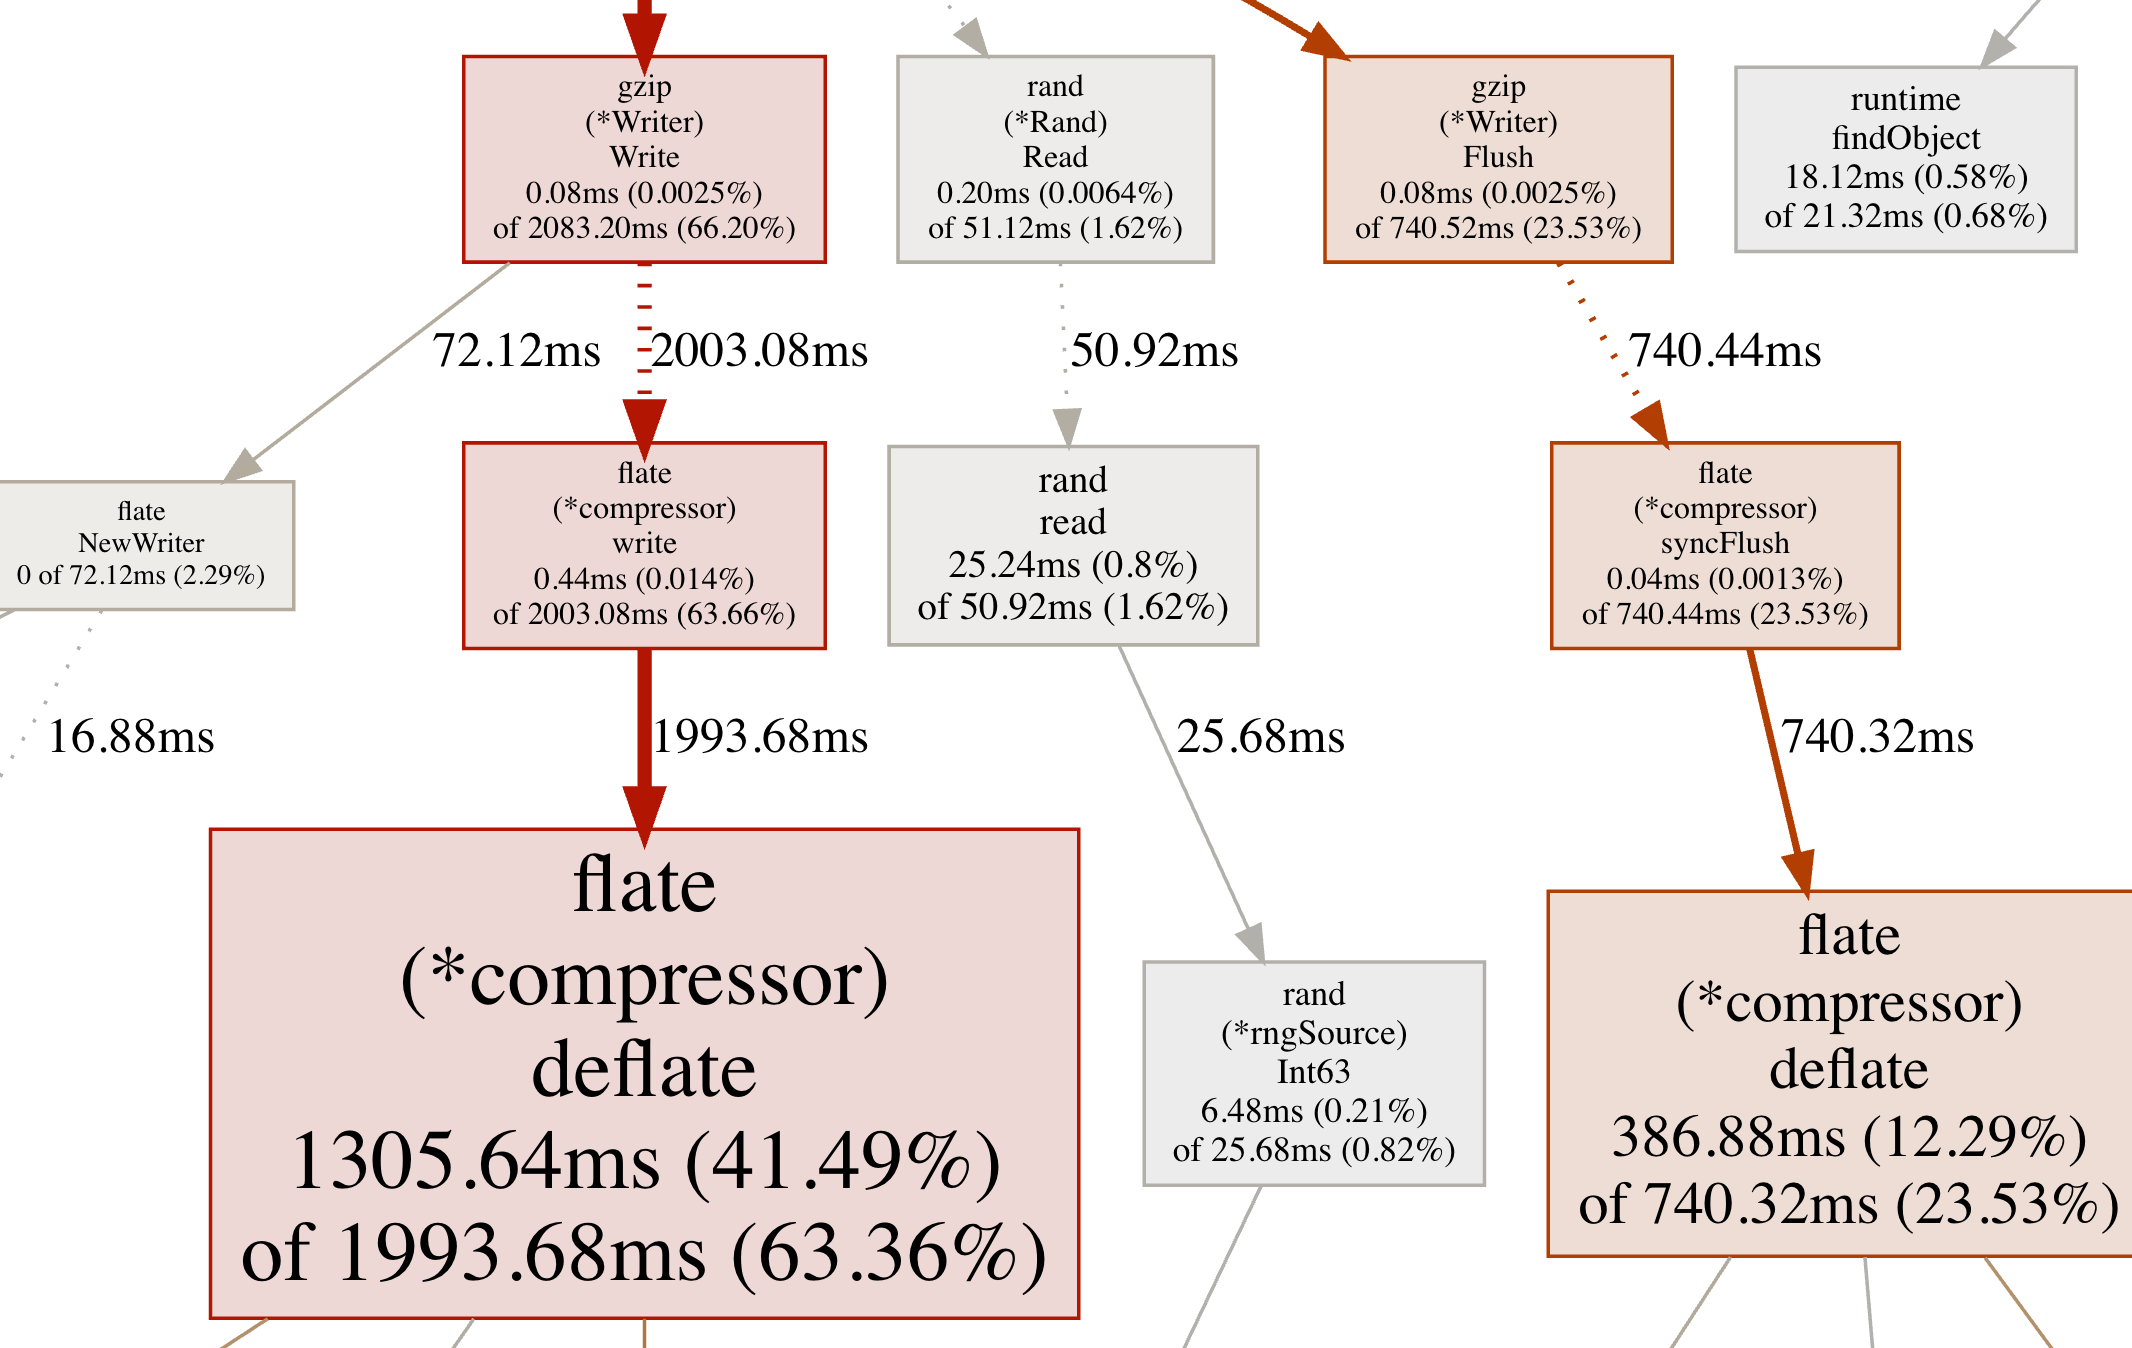
\includegraphics[width=\textwidth]{pprof.png}
    \caption{Пример визуализации профиля при помощи pprof}
    \label{fig:pprof}
\end{figure}

\subsubsection{Flamegraph}
При профилировании крайне важно не только собрать наиболее подходящим образом профиль, но и достаточно информативно визуализировать
полученную информацию. Революционным решением в области визуализации профилей стал Flamegraph \cite{flamegraph}
от евангелиста профилирования Брендара Грига.

\begin{figure}[H]
    \centering
    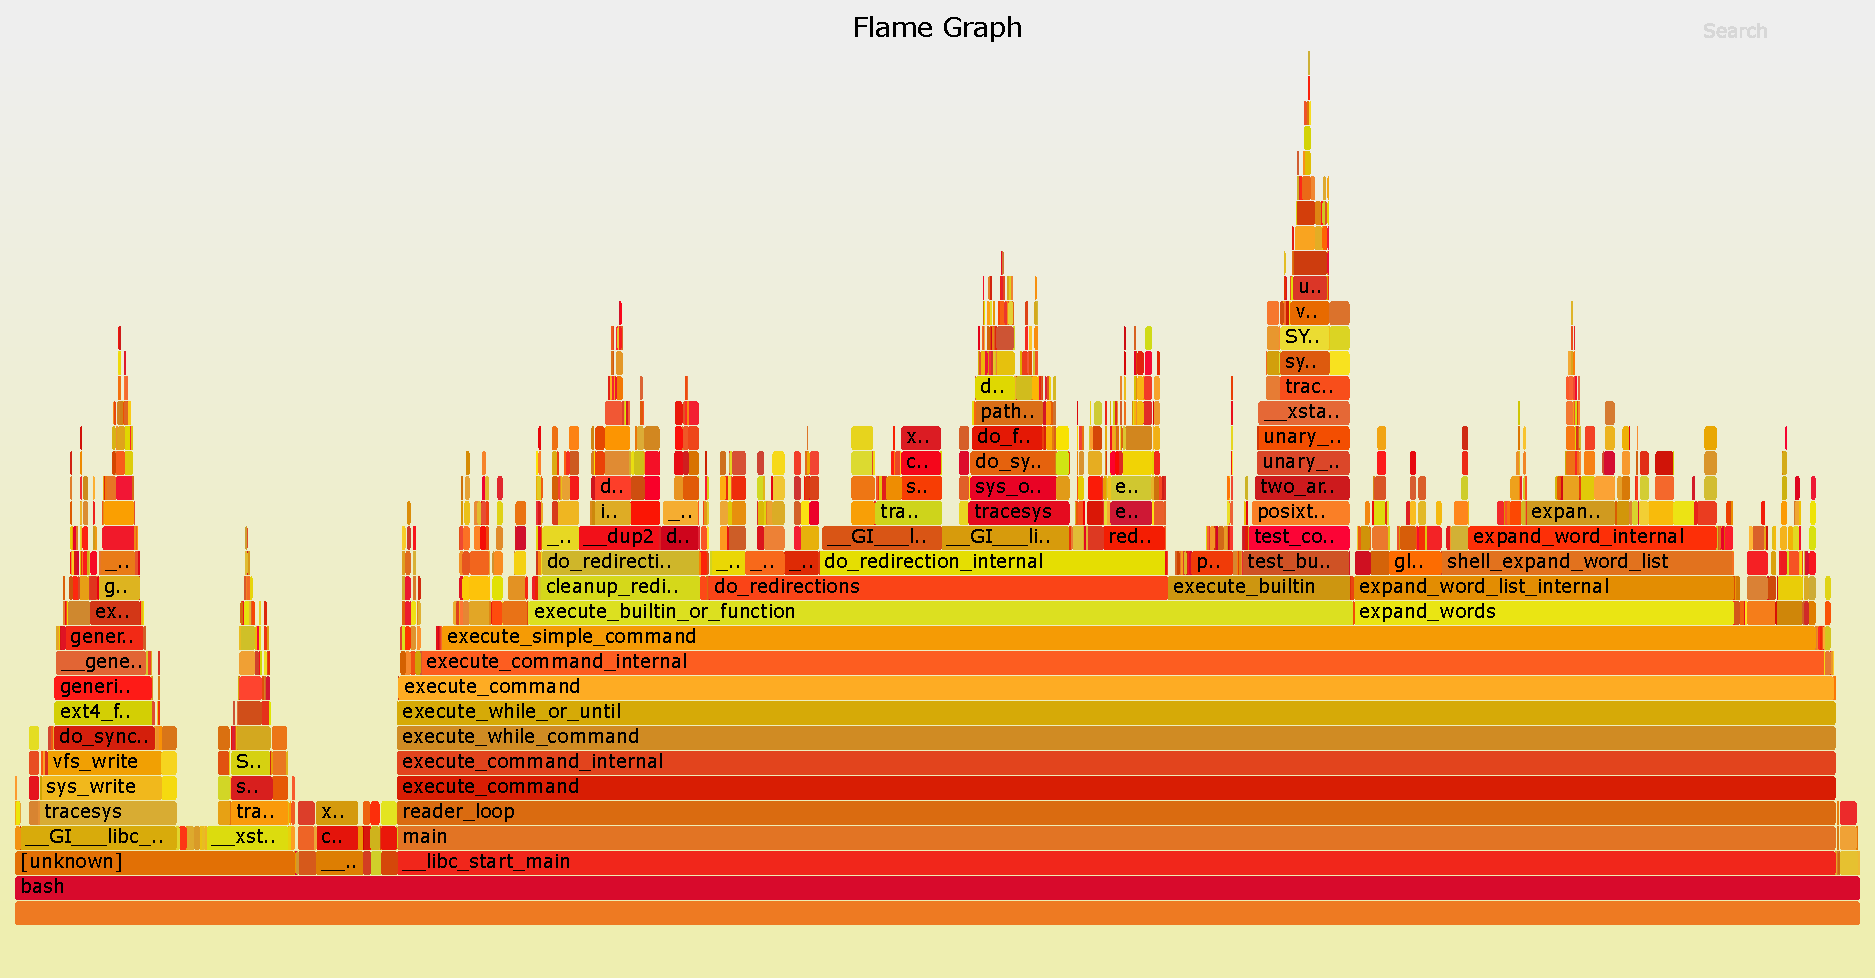
\includegraphics[width=\textwidth]{flamegraph.pdf}
    \caption{Пример визуализации профиля при помощи flamegraph}
    \label{fig:flamegraph}
\end{figure}

Flamegraph строится как префиксное дерево: для каждого собранного семпла стек вызовов добавляется в дерево, где вершинами являются
функции, каждой вершине присвоен вес --- суммарный вес семплов (например, число циклов процессора, приходящихся на этот семпл),
проходящих через нее --- и для каждой вершины определена родительская, за исключением корня.
Таким образом, у корневой вершины вес равен сумме весов всех семплов, а у всех детей --- не больше.

Подобная структура тривиальным образом превращается в пирамидальное изображение, крайне наглядным образом демонстрирующее узкие места системы.Чем шире прямоугольник, соответствующий конкретной функции, тем больше семплов проходят через эту функцию и тем больше эффективно
оптимизировать эту функцию или ее детей.

После появления flamegraph подавляющее большинство профилировщиков стали поддерживать в том или ином виде отрисовку в похожих форматах.
В частности, в интефрейсе pprof появился flamegraph, заметно повышающий удобство использования системы по сравнению с предыдущим решением ---
связным графом зависимостей семплов (рис. \ref{fig:pprof}).

\subsection{Распределенные профилировщики}

\todo{\subsubsection{Google Wide Profiler}}

\subsubsection{Профайлер бедного человека в Яндекс.Рекламе}
На основе poor man's profiler в сервисах Яндекс.Рекламы реализован простой распределенный профилировщик, поддерживающий
построение профилей по A/B экспериментам \cite{pmp:yabs}.
Perforator призван в том числе заменить данное решение.

\todo{\subsubsection{Google Cloud Profiler}}

\todo{\subsubsection{Prodfiler}}

\todo{\subsubsection{Pyroscope}}

\todo{\subsubsection{Parca}}

\subsection{eBPF}
\todo{Про eBPF и пользу, про bcc}
